A path gain must be choosen by modifying the value of r in the command
\begin{lstlisting}
pg = dlmread('path_gains.dat',',',[r,0,r,4])
\end{lstlisting} 
Where r can be any value from 0 to 4.
\\
For r=0, the following figures are obtained
\begin{figure}[!ht]
\centering
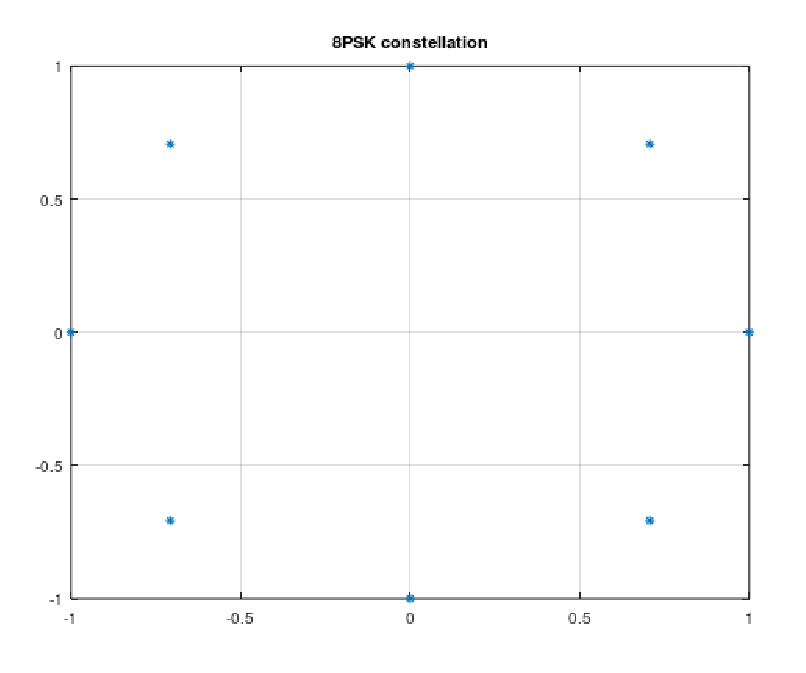
\includegraphics[width=\columnwidth]{./LMS_equalizer_octave/figs/psk.eps}
\caption{8-PSK constellation}
\label{fig:psk}
\end{figure}

\begin{figure}[!ht]
\centering
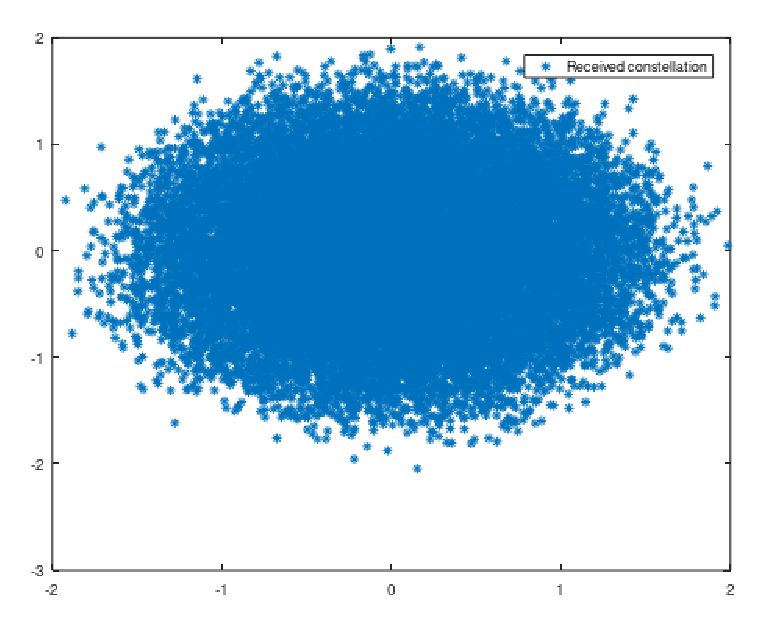
\includegraphics[width=\columnwidth]{./LMS_equalizer_octave/figs/constellation.eps}
\caption{Recieved constellation from the channel}
\label{fig:lms_mse}
\end{figure}

\begin{figure}[!ht]
\centering
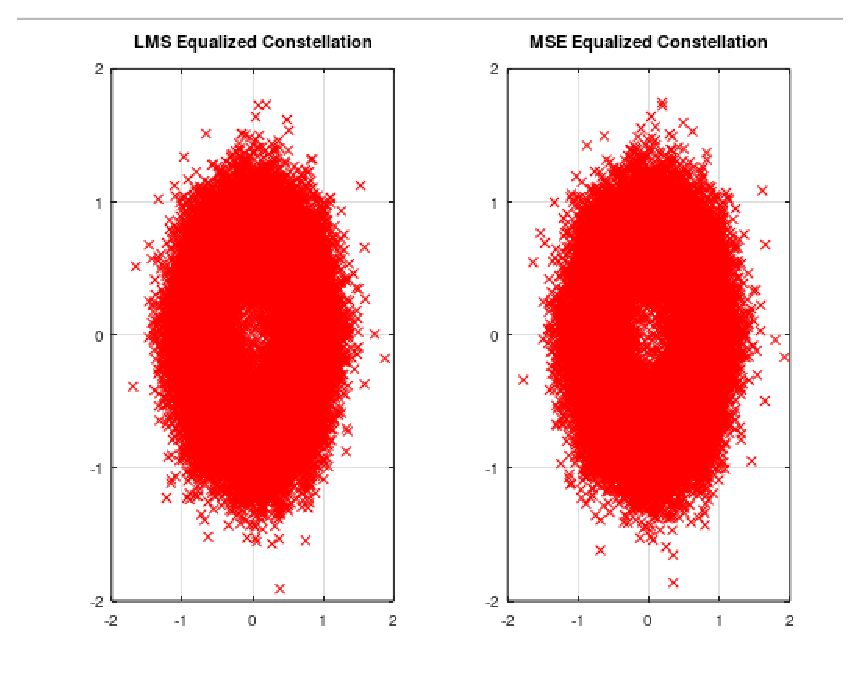
\includegraphics[width=\columnwidth]{./LMS_equalizer_octave/figs/lms.eps}
\caption{LMS and MSE equalized constellation}
\label{fig:lms_mse}
\end{figure}
Hence the code has been executed in octave.
